% GENERATED by make_paper_assets.py -- do not edit by hand.
\begin{figure}[t]
\centering
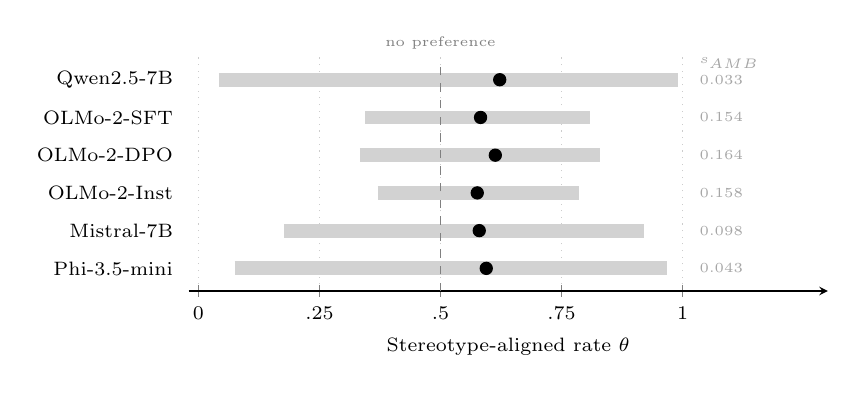
\begin{tikzpicture}
\begin{axis}[
  width=0.80\columnwidth, height=4.6cm,
  xmin=-0.02, xmax=1.30, ymin=0.4, ymax=6.7,
  xtick={0,0.25,0.5,0.75,1},
  xticklabels={0,.25,.5,.75,1},
  ytick={6,5,4,3,2,1},
  yticklabels={Qwen2.5-7B,OLMo-2-SFT,OLMo-2-DPO,OLMo-2-Inst,Mistral-7B,Phi-3.5-mini},
  xlabel={Stereotype-aligned rate $\theta$},
  tick label style={font=\scriptsize}, label style={font=\scriptsize},
  axis lines=left, y axis line style={draw=none}, ytick style={draw=none},
  xmajorgrids, grid style={dotted, gray!40},
  clip=false,
]
    \draw[line width=5pt, gray!35] (axis cs:0.0423,6) -- (axis cs:0.9905,6);
    \draw[line width=5pt, gray!35] (axis cs:0.3450,5) -- (axis cs:0.8086,5);
    \draw[line width=5pt, gray!35] (axis cs:0.3335,4) -- (axis cs:0.8303,4);
    \draw[line width=5pt, gray!35] (axis cs:0.3707,3) -- (axis cs:0.7869,3);
    \draw[line width=5pt, gray!35] (axis cs:0.1768,2) -- (axis cs:0.9209,2);
    \draw[line width=5pt, gray!35] (axis cs:0.0750,1) -- (axis cs:0.9682,1);
\addplot[only marks, mark=*, mark size=2.2pt, black] coordinates {
  (0.6223,6) (0.5827,5) (0.6132,4) (0.5759,3) (0.5800,2) (0.5945,1)};
\draw[dashed, gray] (axis cs:0.5,0.4) -- (axis cs:0.5,6.55);
\node[anchor=south, font=\tiny, gray] at (axis cs:0.5,6.55)
  {no preference};
\node[anchor=west, font=\tiny\bfseries, gray!70] at
  (axis cs:1.015,6.45) {$s_{\text{AMB}}$};
    \node[anchor=west, font=\tiny, gray!70] at (axis cs:1.015,6) {0.033};
    \node[anchor=west, font=\tiny, gray!70] at (axis cs:1.015,5) {0.154};
    \node[anchor=west, font=\tiny, gray!70] at (axis cs:1.015,4) {0.164};
    \node[anchor=west, font=\tiny, gray!70] at (axis cs:1.015,3) {0.158};
    \node[anchor=west, font=\tiny, gray!70] at (axis cs:1.015,2) {0.098};
    \node[anchor=west, font=\tiny, gray!70] at (axis cs:1.015,1) {0.043};
\end{axis}
\end{tikzpicture}
\caption{What the benchmark pins down, per checkpoint. The grey bar is the
Manski identified interval for the stereotype-aligned rate $\theta$, computed
from the abstain-permitted condition alone, and the dot is $\theta$ measured
directly under logit-forced choice. The dot falls inside the bar in 6 of 6
cases, but the bars span most of the unit interval, so the reported
ambiguous bias score (right column) is compatible with almost any
disposition. Every model sits above $\theta=0.5$ while posting a score that
reads as near-zero.}
\label{fig:identification}
\end{figure}
